
\documentclass{article}

\usepackage[utf8]{inputenc}

%Librerias Matematicas
\usepackage{amsfonts}
\usepackage{amssymb}
\usepackage{amsmath}
\usepackage{amsthm}

%Algorithms
\usepackage{algorithm}
\usepackage[noend]{algpseudocode}


\usepackage{soul}%To highligh
\usepackage{fancyhdr}
\usepackage[a4paper]{geometry}
\usepackage{parskip}
\usepackage{changepage}
\usepackage{lipsum}
\usepackage{tikz}
\usepackage{tikzpagenodes}

\usepackage{graphicx}
\usepackage{wrapfig}

\usepackage{adjustbox}
\usepackage{multirow}


\pagestyle{plain}

%Paper Margins and size
\usepackage{geometry}
 \geometry{
 a4paper,
 total={170mm,257mm},
 left=30mm,
 top=20mm,
 right=30mm,
 bottom=20mm
 }

%Page Numeration
\pagestyle{plain}
\thispagestyle{empty}
\clearpage\pagestyle{plain}

%Interline 1.5 (of Word)
\linespread{1.25}

%Ident between 0.5 - 1.25max
\setlength{\parindent}{15pt}

%Math Theorem style
\newtheorem{theorem}{Teorema}
\newtheorem{corollary}{Corolario}[theorem]
\newtheorem{lemma}{Lemma}
\newtheorem*{remark}{Nota}
\theoremstyle{definition}
\newtheorem{definition}{Definición}[section]
\newenvironment{Proof}[1][Proof]
  {\proof[#1]\leftskip=1cm}
  {\endproof}

%Algorithm and PseudoCode
\makeatletter
\def\BState{\State\hskip-\ALG@thistlm}
\makeatother 


\begin{document}

\begin{titlepage}
	\begin{center}
	    
\includegraphics[scale = 0.5]{LogoIngenieriaR.jpg}\\[1.0 cm]
	\end{center}
	
    \vspace*{150pt}
    \centering
    {\Huge
     \textbf{DEUSZUM}
    }
    
	\vspace*{200pt}
	
	
	\begin{minipage}{2in}
		\begin{tabular}{l}
			Terres Escudero, Erik B.    \\
			Zarate Jayo, Gorka   \\
			Zugazaga Alonso, Aritz  \\
			Acha Aristegui, Amaia  \\
			Gago López,Leire  \\
			San Millan Langa, Lander 
		\end{tabular}
	\end{minipage}
	\hfill
	\begin{minipage}{3in}
	\begin{flushright}
	\Large Curso 2019/2020 \\
		\Huge Ing. Informatica\\
		\LARGE Programacion III
	\end{flushright}
		
	\end{minipage}


    
	
\end{titlepage}

\tableofcontents

\clearpage

\section{INTRODUCCIÓN}

DeusZum es una aplicación de gestión de dinero online para la gestión de pagos, proyectos o costes grupales. DeusZum ofrece un sistema seguro de transferencias de forma que el cliente no tenga que preocuparse de que este pasando con su dinero en todo momento.

DeusZum estará implementado en un servidor y daría servicio a los usuarios a través de un programa en Windows y una aplicación en Android. Cada una de ellas implementada para conectarse a un servidor central, en el cual se almacenarán los datos, procesarán las peticiones y se garantizará la seguridad de la información.

El servicio que ofrece DeusZum está dividido en diferentes sectores, algunos puramente económicos y otros de análisis de la conducta o de las transacciones. El servidor ejecutara todas las peticiones de los usuarios y devolverá la información que se haya solicitado. Toda la información mientras se enviá se encontrara encriptada para la seguridad del usuario.

\section{FORMA DE TRABAJO}


\subsection{Division del trabajo}

Para la realización del proyecto, hemos optado por la división del trabajo en grupos con temáticas separadas. Los dos grupos tendrán que trabajar en una categoría central entre IA y Seguridad, y, trabajar en una parte de la implementación y algoritmia. Las categorías y subcategorías serian las siguientes:

\begin{enumerate}
    \item \textbf{Implementacion} \begin{itemize}
        \item Implementación del Server
        \item Implementación del cliente Windows
        \item Implementación del cliente Android
    \end{itemize}
    \item \textbf{IA} \begin{itemize}
        \item Data Analysis
        \item Clustering
    \end{itemize}
    \item \textbf{Seguridad} \begin{itemize}
        \item Databases
        \item Encriptación
        \item Conexiones seguras
    \end{itemize}
\end{enumerate}



Cada uno de los grupos tendra un conjunto de tareas las cuales se diviran en \textit{tareas principales} y \textit{tareas secundarias}. Las tareas principales son aquellas a las que se les daran prioridad y buscamos que esten terminadas a la hora de terminar el proyecto. Las tareas secundarias son aquellas que no tienen tanta importancia y que se empezaran una vez se vallan acabando las tareas principales.

A su vez, las tareas estaran numeradas segun importancia, dificultad y tiempo de trabajo con el fin de poder establecer un orden de prioridad para que su progreso haga que el proceso de construccion del proyecto sea relativamente optimo y de forma que su estructura no se vea afectada por software anterior.

Por ultimo, hay un sector no especializado que trata los temas de algoritmia sobre como handlear la forma de minimizar el total de pagos que hay realizar en forma de peticiones. Este algoritmo estara pensado en forma de algoritmo greedy al tener complejidad $O(n)$, pero en caso de que consigamos un algoritmo que no dependa de combinatorial algorithms o complejidades exponenciales para encontrar el minimo numero de pagos, tal vez aniadamos la opcion. Por ahora no sabemos como de rentable resultaria este algoritmo, ni tampoco sabemos ninguna upperbound del numero de movmientos que sea inferior a $n$ aproximadamente. Esto se mostrara en la bibliografia final o en la documentacion sobre el software.

El apartado de algoritmia se dividira segun convenga, aunque se mostrara dentro de la documentacion quien ha hecho que tareas y como ha resuelto los problemas.
\subsection{Error Handling}

Para evitar errores que afecten al codigo a nivel global, hemos optado por utilizar github y hacer que cada miembro del grupo tenga su propia cuenta. Los errores, comentarios y todo se enviarian a traves de github excepto la informacion mas urgente que se enviaria a traves de un grupo de whatsapp o telegram/discord en si defecto.

\subsection{Preparacion del temario}

Para la preparacion del temario que queremos trabajar en el trabajo hemos optado por utilizar un conjunto de libros que consideramos basicos para las personas que no tienen mucha experiencia y utiles/importantes para las personas que tengan un cierto control en ciertos aspectos. Esta lista de libros se encontrara en el apendice de este documento categorizada.

\section{PLANIFICACION}
23 Reunion Inicial
8 de octubre	E1. 
29 de octubre	E2. Fase I del proyec to
26 de noviembre	E3. Examen parcial
10 de diciembre	E4. Fase II del proyecto
13 de diciembre	E5. Informe de desarrollo

\subsection{Entrega de la Idea}

Propuesta de proyecto y planificación

\begin{itemize}
    \item Reparto de tareas
    \item Desarrollo de las ideas basicas
    \item Preparacion de la bibliografia
    \item 
\end{itemize}

\begin{itemize}
    \item Crear el Servidor Generico
    \item Crear la aplicacion Desktop Funcional sin muy grafico
    \item Crear una aplicacion android funcional sin muy grafico
    \item planificacion per
\end{itemize}
\subsection{Fase 1}
29 de octubre

\begin{itemize}
    \item 
\end{itemize}


\subsection{Fase 2}
diciembre
\subsection{Informe de Desarrollo}
dic
\subsection{Entrega Final}
enero



\section{Implementacion de Server}


La implementacion del Server sera una implementacion sencilla de un serversocket con la capacidad de extension de funcionalidades. Incluso tal vez no necesitar modificar el codigo del server per se para la ampliacion de su funcionalidad. 

Los sockets del servidor tendrian una estructura tal que:
\begin{enumerate}
    \item Conseguir acceder a la cuenta de un usuario.
    \item Comprobar que el usurio existe y verificar que la contrasenia es correcta.
    \item Verificar que no ha habido un abnormal comportation.
    \item Devolverle un hash que representa su sesion actual en el servidor.
    \item En caso de que quiera guardar la sesion, devolverle otro hash que represente su sesion y guardar en el servidor que esa sera su sesion activa.
    \item Este hash debera ser modificado cada x tiempo.
\end{enumerate}

\begin{wrapfigure}{R}{0.4\textwidth}
\centering
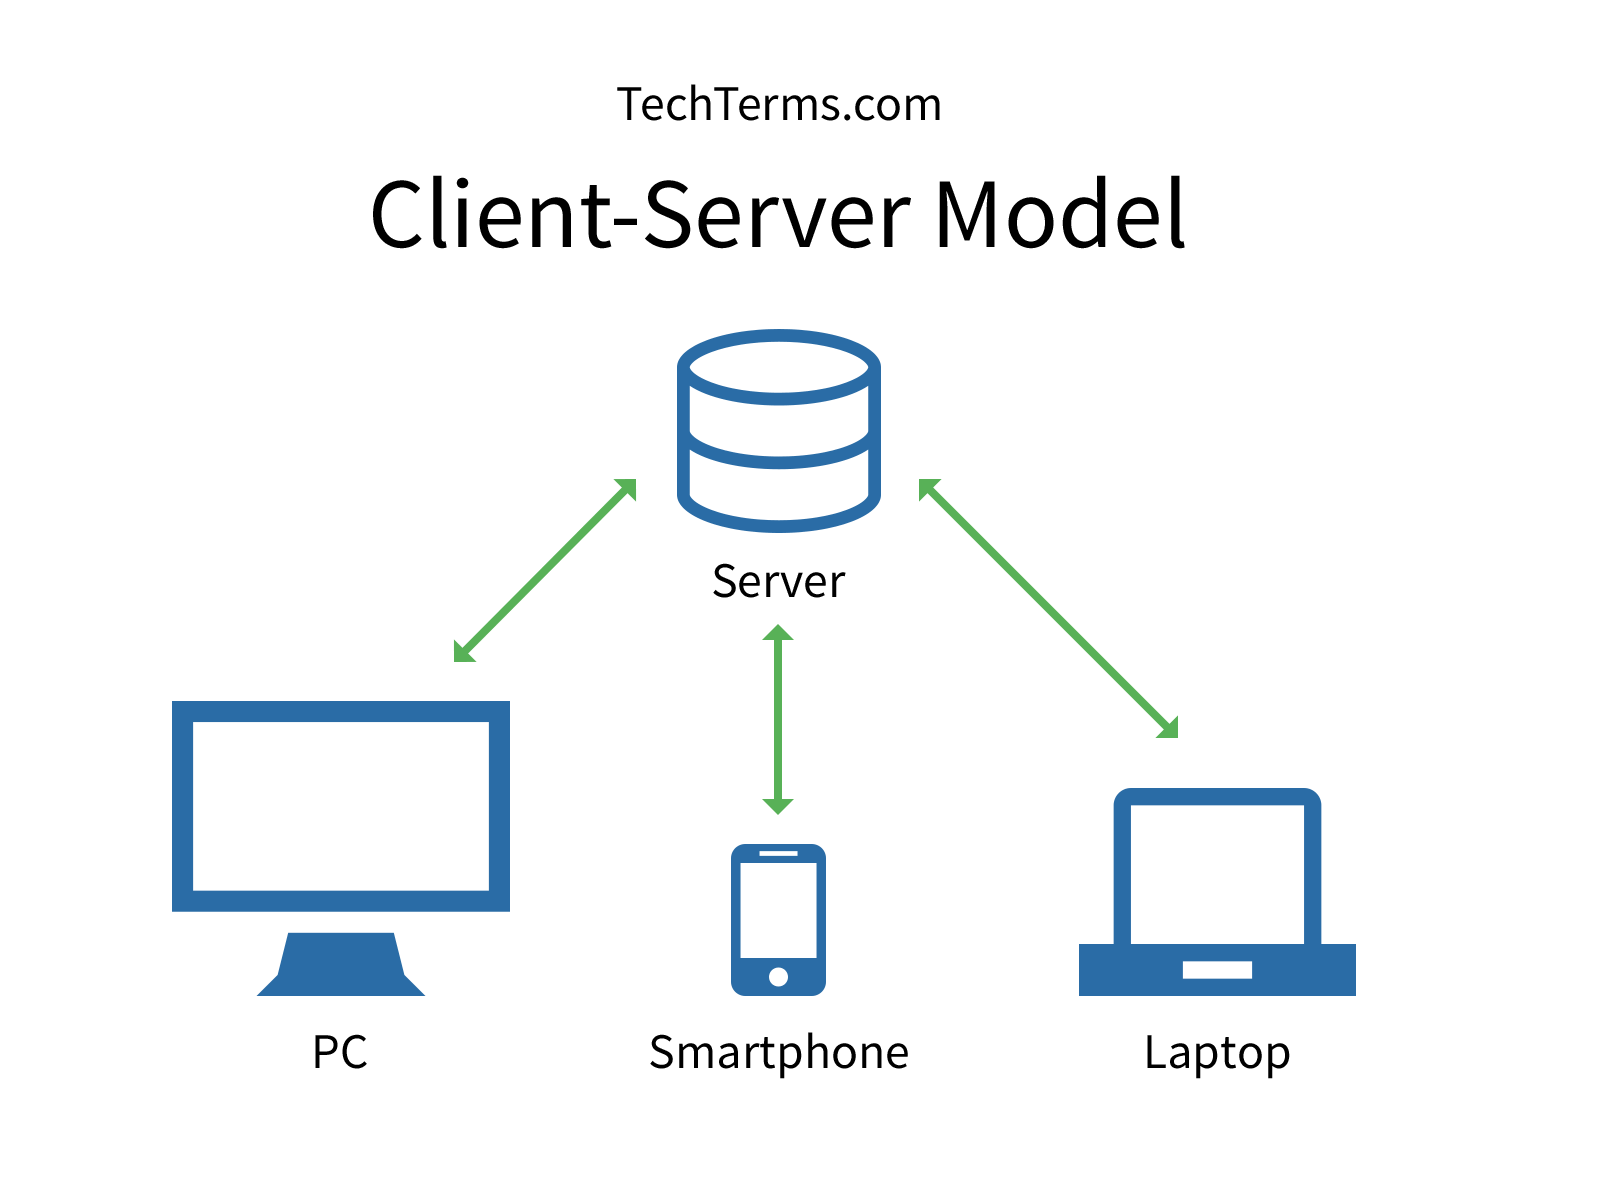
\includegraphics[width=0.4\textwidth]{pics/serverclient.png}
\caption{Modelo del Servicio.}
\end{wrapfigure} 

Los sockets de funcionalidad estaran compuestos por un comando, luego el servidor devolvera un codigo hash de sesion activa y a continuacion el cliente enviara toda la informacion con el hash como cabecera.

Estos hash se enviaran a traves de la web mediante un sistema de criptografia implementado por nuestro equipo y, por otro lado, plantearemos un metodo mas seguro para mostrar la capacidad de implementar metodologias mas serias o profesionales.

El ServerHandler no debera ser modificado cada vez que se aniada un nuevo codigo de funcionalidad en el server. Para manejar esto, hemos pensado en hacer que el serverhandler funcione mediante un arbol Autobalanceado (AVL o Black Red por ejemplo) que se genera al inicio de la sesion del servidor y que despues, en cada peticion, el serverhandler simplemente busque cual de las hojas es y luego ejecute otra funcon que se encuentre en algun otro lado del codigo. Este arbol se generaria mediante una base de datos que contenga el conjunto de funcionalidades y la funcion asociada.



\section{Implementacion de Desktop}

La aplicacion de escritorio sera puramente una aplicacion que sirva como cliente para el servidor y que sirva para enviar sockets y representar de forma visual todos los comandos que se podran enviar al servidor.

La implementacion del software de Desktop se basará en tres valores principales: comodidad, sencilles y completitud. Buscamos crear una aplicacion que satisfaga todas las necesidades de los usuarios, manteniendo a su vez la sencillez que supone un software minimalista y con el apoyo de IA.




\section{Implementacion de Android}




\section{IA}

El apartado de IA de DeusZum se basara puramente en el analisis de la conducta de los usuarios dentro de la aplicacion con el unico fin de garantizar su seguridad.

Las tareas que queremos hacer en el apartado de IA son las siguientes:

\begin{itemize}
    \item Analisis de los movimientos economicos de los clientes.
    \item Analisis del tracking de las direcciones de las transacciones de los clientes.
    \item Analisis conductual del cliente dentro de la apliacion.
    \item Prediccion de los clientes dentro de la apliacion.
\end{itemize}


\subsection{Analisis de los movimientos}

\subsection{}

\section{DATA ANALYSIS}

\begin{itemize}
    \item Clustering
    \item Analisis de mercado
\end{itemize}

\section{SEGURIDAD}

\begin{itemize}
    \item Encriptacion de todas las conexiones.
    \item Capacidad de trackeo del historial de conexiones
\end{itemize}

\subsection{Encriptacion de los codigos de los sockets}

A la hora de enviar la informacion al servidor, nos parece importante que no pueda exitir un sniffer que robe la informacion de nuestros clientes como puede ser el hash de la sesion o como puede ser el usuario y contrasenia. Para evitar esto, necesitaremos que nuestra informacion se envia encriptada con algun tipo de codigo decriptable asi como con un conjunto de informacion basura para evitar que a base de fuerza bruta en codigos cortos se pueda adivinar lo que ciertos codigos encriptados hagan.

Para solucionar este problema, el grupo de seguridad se encargara de estudiar el funcionamiento de ciertos tipos de encriptacion inyectiva o biyectiva y analizaran algunos metodos para aumentar la seguridad del algoritmo de encriptacion que deberan crear.

Sea $A$ el alfabeto, $f : A^n \to A^w$ la funcion de encriptacion con $n \in \mathbb{N}$.Las condiciones que establecemos ahora sobre el algoritmo de enriptacion seran las siguientes:

\begin{enumerate}
    \item $f$ sera inyectiva.
    \item $\mathbb{P}\left(|f(x)|=|x|\right) \to 0$ cuando $n \to \infty$.\, siendo $x \in A^n$.
    \item $f$ no pueda ser roto por analisis de frecuencia.
\end{enumerate}

\subsection{Trackero de los pagos}

\section{DATABASES}


Las tareas dentro de este subapartado se dividiran en 2, la de creacion y organizacion inicial de las bases de datos y la segunda, la de optimizacion de las bases de datos y su respectivo ajuste de seguridad con el fin de evitar ciertos tipos de ataque como las SQL Inyection o las code execution.


\begin{itemize}
    \item Optimizacion de las bases de datos
\end{itemize}

\section{DIVISION DEL TRABAJO}


\begin{tabular}{|c|c|}
    \hline Grupo 1 & Grupo 2 \\
    \hline Implementacion Desktop & Implementacion Server \\
    Implementacion App & IA \\
    Seguridad & Data Mining \\
    Database 2 & Database 1 \\
    \hline
\end{tabular}

\begin{tabular}{|c|c|}
    \hline
    Grupo 1  & Grupo 2 \\
    \hline
    Aritz & Erik \\
    Leire & Lander \\
    Gorka & Amaia \\
    \hline
\end{tabular}




\section{CONCLUSIÓN}


\section{LIBRERIAS}

\begin{enumerate}
    \item \textbf{DeepLearning4J}: Usaremos esta libreria para la implementacion de redes neuronales y ejecutarla. A su vez, esta libreria permite el uso de tensores para la representacion de datos, lo cual nos puede ser util.
\end{enumerate}

\section{LIBROS}

\subsection{Java}

\subsection{Android}

\subsection{Server}

\subsection{IA}

\subsection{Data Analisys}

\subsection{Seguridad}


\begin{enumerate}
    \item 
\end{enumerate}

\begin{thebibliography}{9}
\bibitem{Example}
Autor1, Autor2. (2002) \textit{Nombre del articulo}, Lugar de publicación

\end{thebibliography}

\end{document}